
\documentclass[11pt,a4paper]{article}
\usepackage[utf8]{inputenc}
\usepackage{amsmath}
\usepackage{amsfonts}
\usepackage{amssymb}
\usepackage{enumerate}
\usepackage{graphicx}
\usepackage{enumitem}



\title{Lab 02\\Arquitectura de Computadores \\ \Large{Sección 2}}
\author{Joaquín Ramírez}
\date{Mayo 04, 2020}
\begin{document}
\maketitle
Nota: Todos los \textit{time scales} de los \textit{test benches} son $\frac{1ns}{1ns}$. Además, en cada \textit{test bench} se genera un archivo \textit{.vcd}, el cual será ejecutado en \textit{GTKWave}.
\begin{enumerate}
\item Será implementado en el ejercicio 2.a
\item	MUX
\begin{enumerate}[label=(\alph*)]
\item Implementación de un 2-to-1 MUX de 16-bits. La implementación es igual que un MUX 2x1 de 1 bit. En el \textit{.v}, el \textit{output} está en función del $select$. Si éste último es $0$, entonces se le asignará a $y$ el valor de $a$. En el otro caso, cuando $s = 1$, $y = b$.
\begin{figure}[h!]
\centering
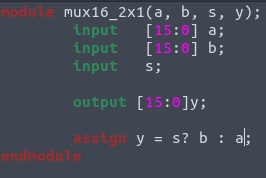
\includegraphics[scale=0.6]{16_2x1MUX_1.png} 
\end{figure}

El \textit{test bench} analiza dies tiempos diferentes. El $select$ varía cada dos tiempos, para que dentro de ese intervalo se pueda observar cómo en cada tiempo el \textit{output} cambia entre $a$ y $b$. Los valores iniciales son: $a = 1111000011110000$ y $b = 0000111100001111$. Cada tiempo, $a$ disminuye en $1$, y cada dos tiempos $b$ se incrementa en $1$.
\pagebreak

\begin{figure}[h!]
\centering
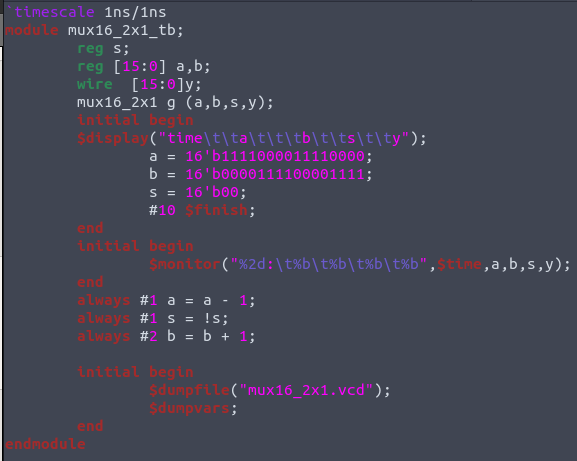
\includegraphics[scale=0.35]{16_2x1MUX_2.png} 
\end{figure}

La tabla de verdad obedece el comportamiento planteado.

\begin{figure}[h!]
\centering
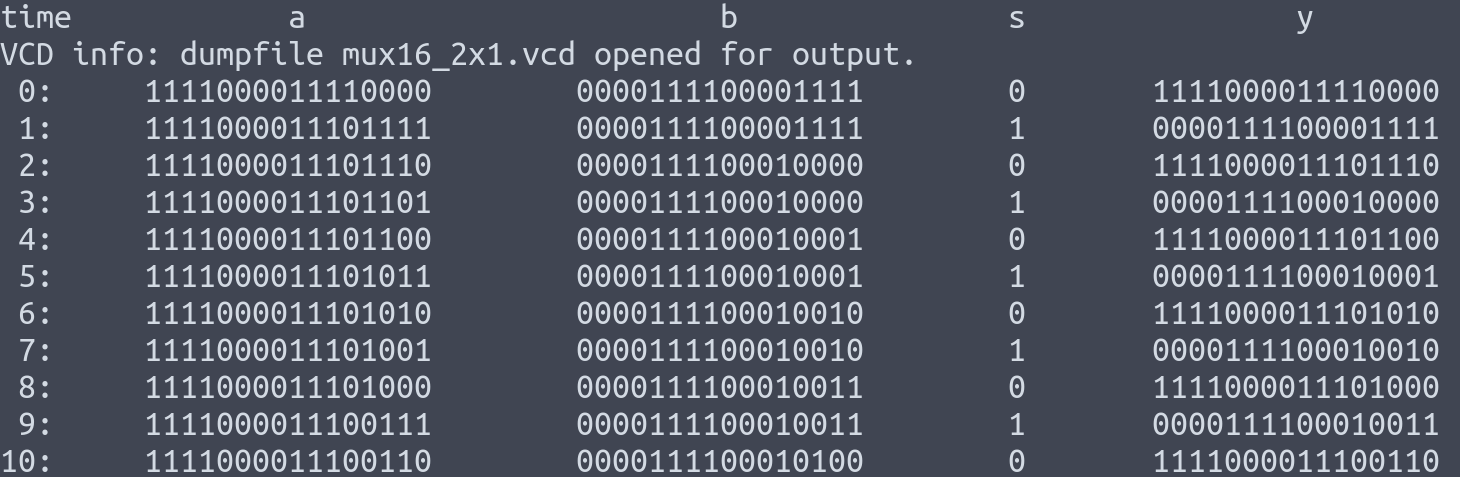
\includegraphics[scale=0.2]{16_2x1MUX_3.png} 
\end{figure}
A través de los \textit{waveforms} queda más claro el cambio de valores de $y$, entre $a$ y $b$.
\begin{figure}[h!]
\centering
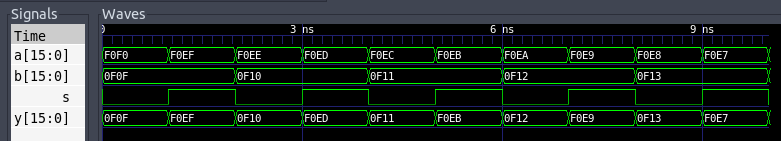
\includegraphics[scale=0.4]{16_2x1MUX_4.png} 
\end{figure}

\item Implementación de un 8-to-1 MUX de 16-bits.Se crearon \textit{small modules} que fueron integrados en un \textit{top}. Para la construcción del sistema se partió del siguiente sistema.
\pagebreak
\begin{figure}[h!]
\centering
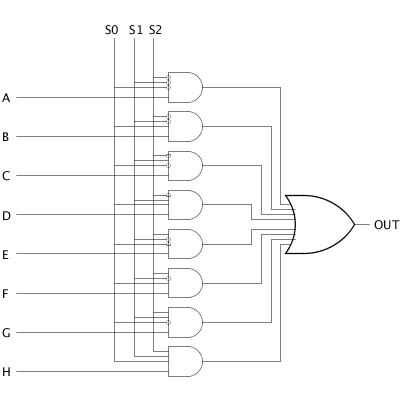
\includegraphics[scale=0.5]{mux8x1diagram.png} 
\end{figure}

El módulo NOT se encarga de negar a cada $select$, para que se puedan formar todas las combinaciones. El módulo niega un input de 1 bit.
\begin{figure}[h!]
\centering
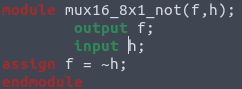
\includegraphics[scale=0.5]{16_8x1MUX_3.png} 
\end{figure}

Ya que hay $3 \ selects$, entonces habrán $2^ 3= 8$ posibles combinaciones. Es así que hay una compuerta AND para cada una, la cual se activará únicamente con un determinado input de $selects$. El módulo AND valida que la combinación  de $selects$ sea ``high". De ser el caso, el $wire output$ será igual al valor del bus de 16 bits. Si no, será un cero lógico de 16 bits. 
\begin{figure}[h]
\centering
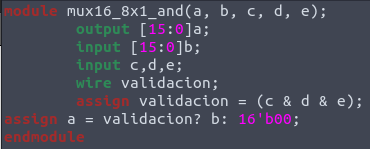
\includegraphics[scale=0.5]{16_8x1MUX_2.png} 
\end{figure}

Todos los \textit{wire outputs} previos se juntan en un único or de $8 inputs$. El $output$ final tomará el valor del $wire$ cuya combinación de $selects$ se ``activó".
\pagebreak 
\begin{figure}[h!]
\centering
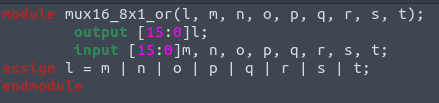
\includegraphics[scale=0.7]{16_8x1MUX_1.png} 
\end{figure}

Se juntan los módulos previos en el $.v$, el cual está basado en el diagrama de MUX 8x1 anterior.
\begin{figure}[h!]
\centering
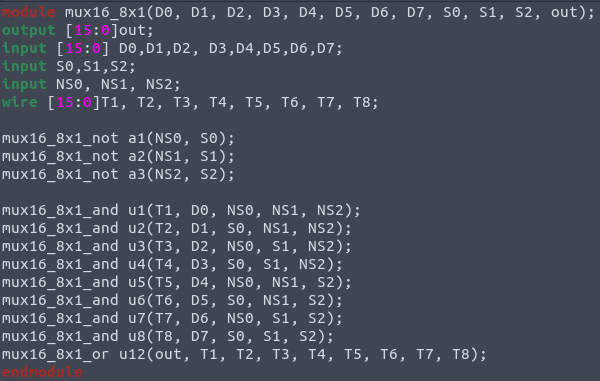
\includegraphics[scale=0.4]{16_8x1MUX_4.png} 
\end{figure}

En el \textit{test bench} se asignan valores diferentes a cada uno de los 8 $16-bit inputs$. Dentro de un intervalo de 8 tiempos se permutan los $selects$, para ver que el $output$ es igual a un diferente input en cada ocasión.
\begin{figure}[h!]
\centering
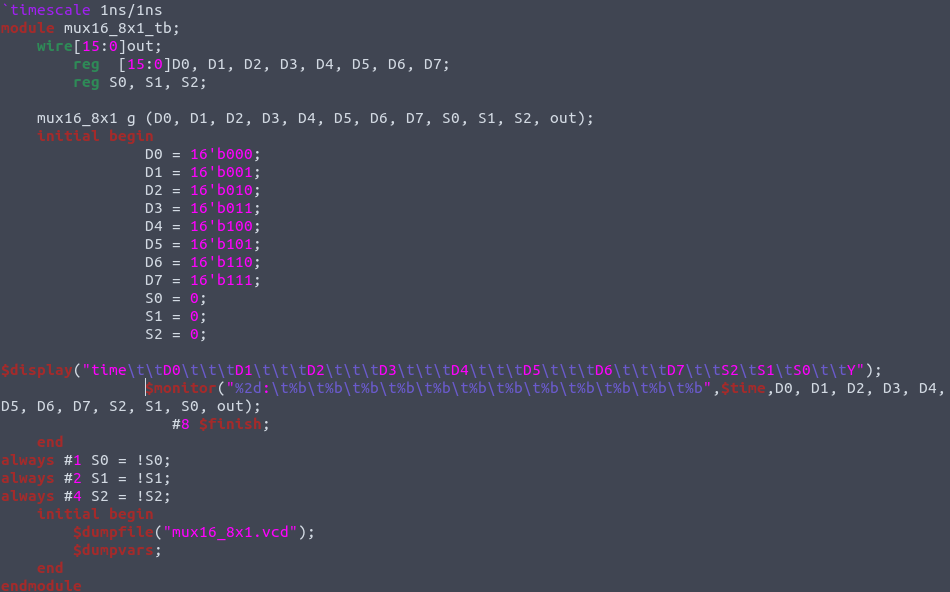
\includegraphics[scale=0.35]{16_8x1MUX_5.png} 
\end{figure}

La tabla de verdad confirma lo descrito, cada tiempo el $output$ corresponde a un único $input$.
\begin{figure}[h!]
\centering
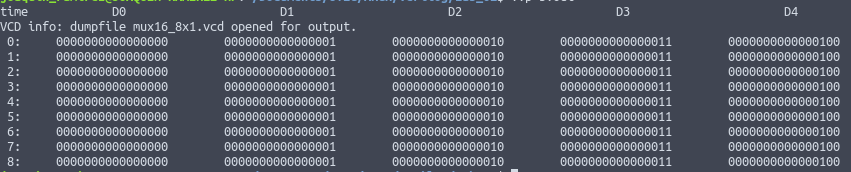
\includegraphics[scale=0.38]{16_8x1MUX_61.png} 
\end{figure}
\begin{figure}[h!]
\centering
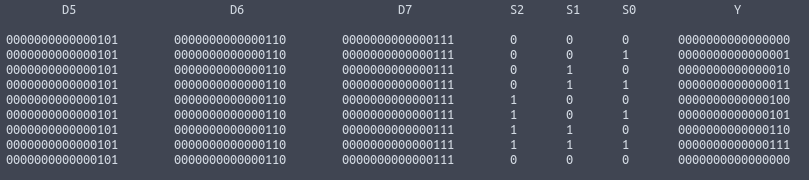
\includegraphics[scale=0.4]{16_8x1MUX_62.png} 
\end{figure}

Los \textit{waveforms} permiten ver con mayor claridad la asignación al $output$ de un diferente $input$ en cada tiempo.
\begin{figure}[h!]
\centering
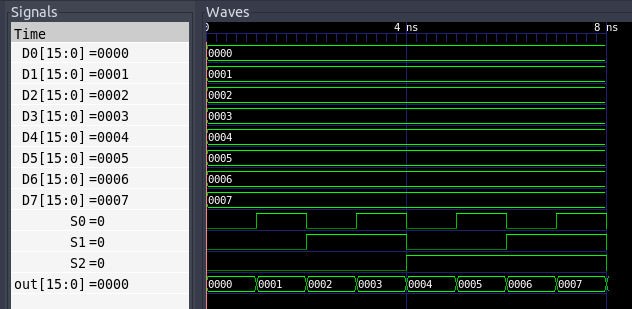
\includegraphics[scale=0.45]{16_8x1MUX_7.png} 
\end{figure}
\item Implementación de un 16-to-1 MUX de 16-bits. La elaboración de este sistema sigue la misma idea del diagrama del MUX 8x1, pero varían ciertas cosas.

El módulo NOT continúa devolviendo la negación de 1 bit.
\begin{figure}[h!]
\centering
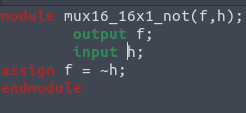
\includegraphics[scale=0.5]{16_16x1MUX_3.png} 
\end{figure}

Ya que ahora hay 4 $selects$, entonces existirán $2^4 = 16$ posibles combinaciones. De esta manera, el AND tiene que validar 4 $selects$ de 1 bit cada uno. Si la combinación es ``high", entonces el \textit{wire output} será igual que el input, si no, un 0 de 16 bits.
\pagebreak
\begin{figure}[h]
\centering
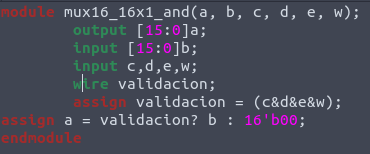
\includegraphics[scale=0.7]{16_16x1MUX_2.png} 
\end{figure}

En este caso, el OR tiene 16 \textit{wire outputs} anteriores, de los cuales dejará pasar a aquel cuya combinación de $selects$ fue ``high".

\begin{figure}[h!]
\centering
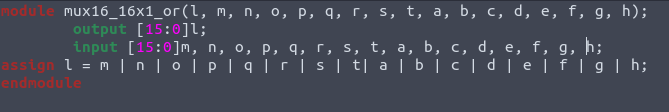
\includegraphics[scale=0.4]{16_16x1MUX_1.png} 
\end{figure}

Se juntan los módulos previos en el \textit{.v (top)}, que sigue la misma idea que el desarrollado para el MUX 8x1, solo que aumentando un $select$.
\begin{figure}[h!]
\centering
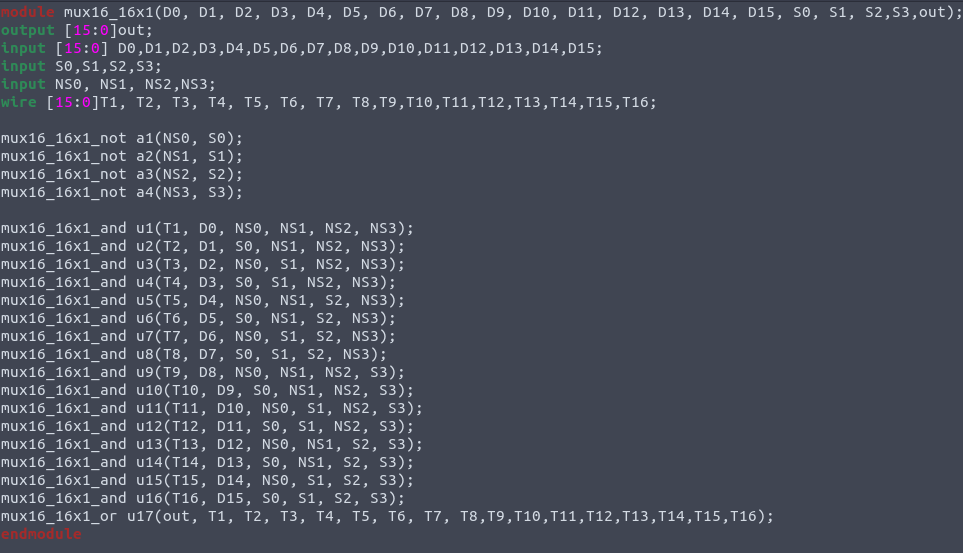
\includegraphics[scale=0.4]{16_16x1MUX_4.png} 
\end{figure}

En el \textit{test bench} se asignan valores únicos para cada input, y durante 16 tiempos, se generan todas las combinaciones de $selects$.
\pagebreak
\begin{figure}[h!]
\centering
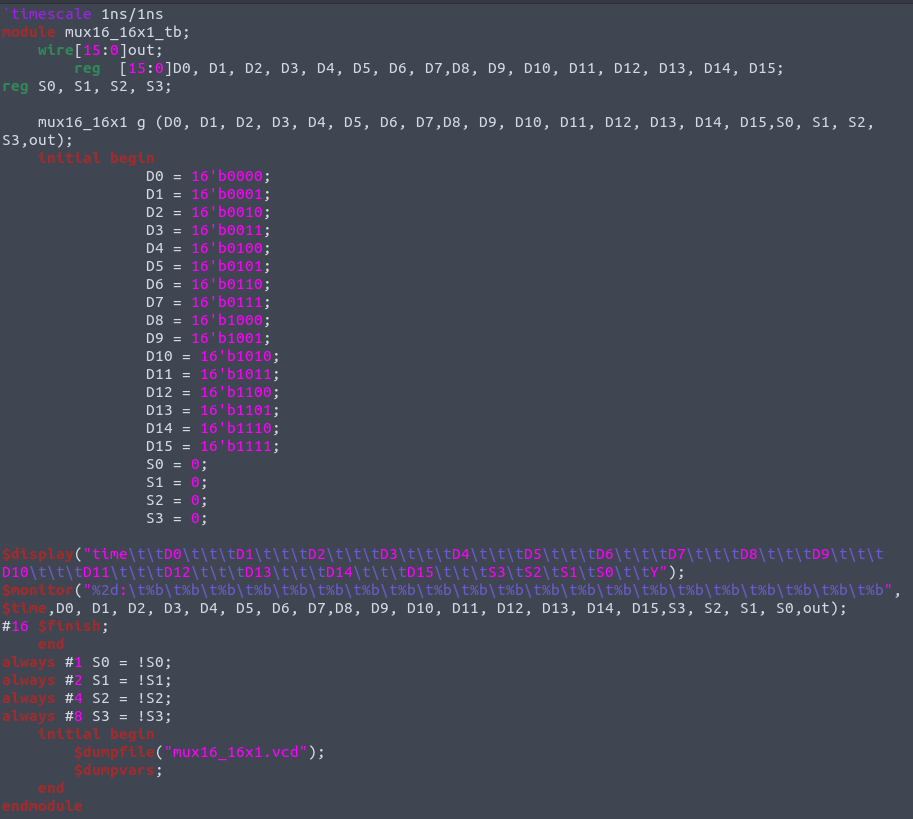
\includegraphics[scale=0.4]{16_16x1MUX_5.png} 
\end{figure}

La tabla de verdad corrobora lo planteado: el \textit{output Y} varía en valores conforme cambian los $selects$.
\begin{figure}[h!]
\centering
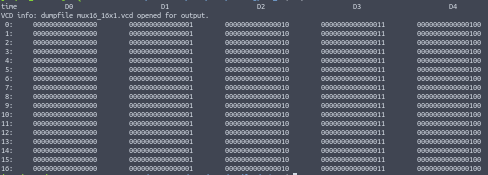
\includegraphics[scale=0.7]{16_16x1MUX_61.png} 
\end{figure}

\pagebreak
\begin{figure}[h!]
\centering
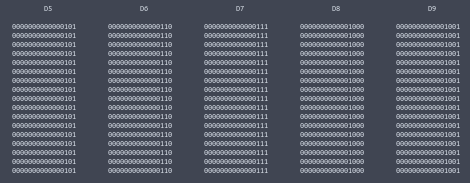
\includegraphics[scale=0.7]{16_16x1MUX_62.png} 
\end{figure}

\begin{figure}[h!]
\centering
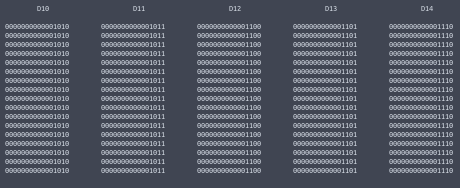
\includegraphics[scale=0.7]{16_16x1MUX_63.png} 
\end{figure}

\begin{figure}[h!]
\centering
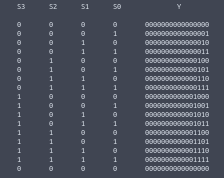
\includegraphics[scale=0.7]{16_16x1MUX_64.png} 
\end{figure}
\pagebreak
Los \textit{waveforms} ilustran mejor la variación del \textit{output Y}.
\begin{figure}[h!]
\centering
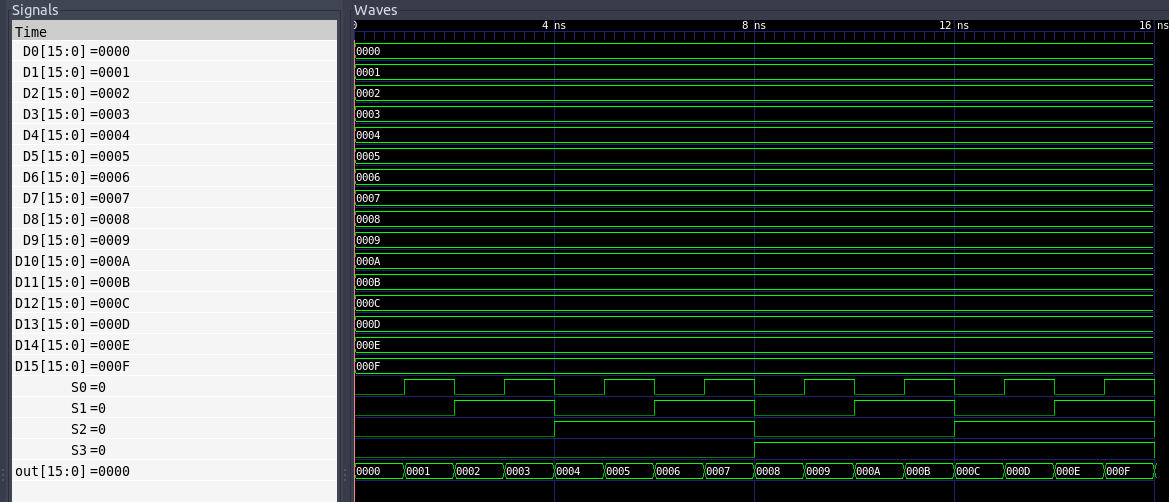
\includegraphics[scale=0.3]{16_16x1MUX_7.png} 
\end{figure}
\end{enumerate}

\item DEMUX
\begin{enumerate}[label=(\alph*)]
\item Implementación del DEMUX 1-to-2 de 16-bits. Se elaboró todo en el $.v$, pues no tenía mucha complejidad. A cada $output$ se le asigna el valor del input si y solo si un determinado select está presente. A $y0$ se le asigna $D0$ si $s=0$, y a $y1$ se le asigna $D0$ si $s = 1$. Cuando el $select$ no le corresponde al $output$, se le asigna un 0 de 16 bits.
\begin{figure}[h!]
\centering
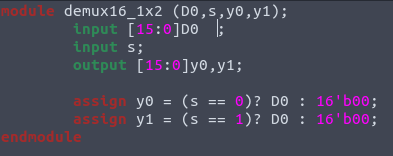
\includegraphics[scale=0.5]{16_1x2DEMUX_1.png} 
\end{figure}

En el \textit{test bench} se asignan ún valor inicial $D0 = 16'b01$. Cada tiempo, por 6 tiempos, D0 aumentará en 1, y el $select$ se negará, para ver que los outputs toman distintos valores dependiendo del valor del $select$.
\pagebreak
\begin{figure}[h!]
\centering
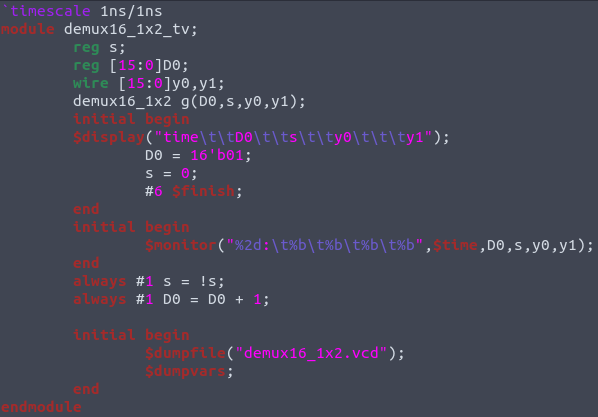
\includegraphics[scale=0.4]{16_1x2DEMUX_2.png} 
\end{figure}

La tabla de verdad confirma lo planteado.
\begin{figure}[h!]
\centering
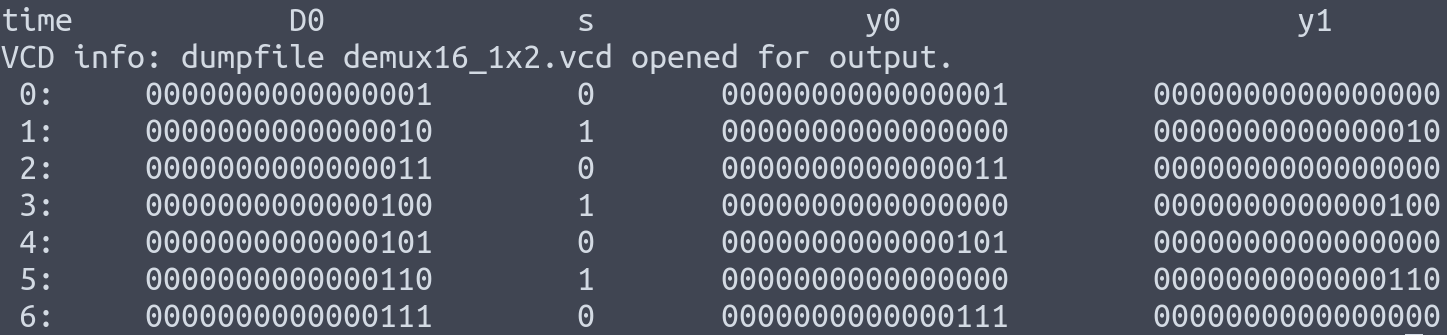
\includegraphics[scale=0.25]{16_1x2DEMUX_3.png} 
\end{figure}

A través de los \textit{waveforms} se puede ver cómo el valor de $D0$ se le asigna a un determinado output según el valor de $s$.
\begin{figure}[h!]
\centering
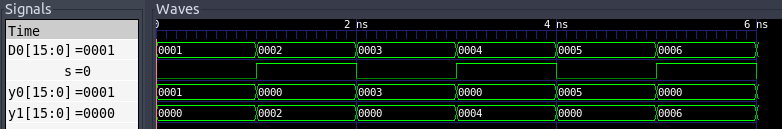
\includegraphics[scale=0.5]{16_1x2DEMUX_4.png} 
\end{figure}
\item Implementación del DEMUX 1-to-8 de 16-bits. De acuerdo a la misma idea anterior, si una determinada combinación de $selects$ se presenta para determinado output, entonces a éste se le asigna el valor de D0. De lo contrario, se le asigna un 0 de 16 bits. En este caso, el $select$ es un bus de 3 bits, con el que se pueden generar $2^3 = 8$ posibles combinaciones.
\pagebreak
\begin{figure}[h!]
\centering
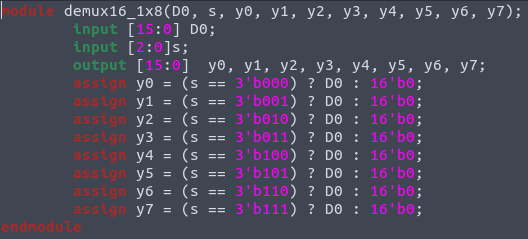
\includegraphics[scale=0.5]{16_1x8DEMUX_1.png} 
\end{figure}

En el \textit{test bench} se asignan ún valor inicial $D0 = 16'b01$. Se analizan 8 tiempos, dentro de los cuales cada se generarán todas las combinaciones de 3 bits del $select$. Esto permitirá ver que en cada tiempo, solo un output tendrá el valor de $D0$.
\begin{figure}[h!]
\centering
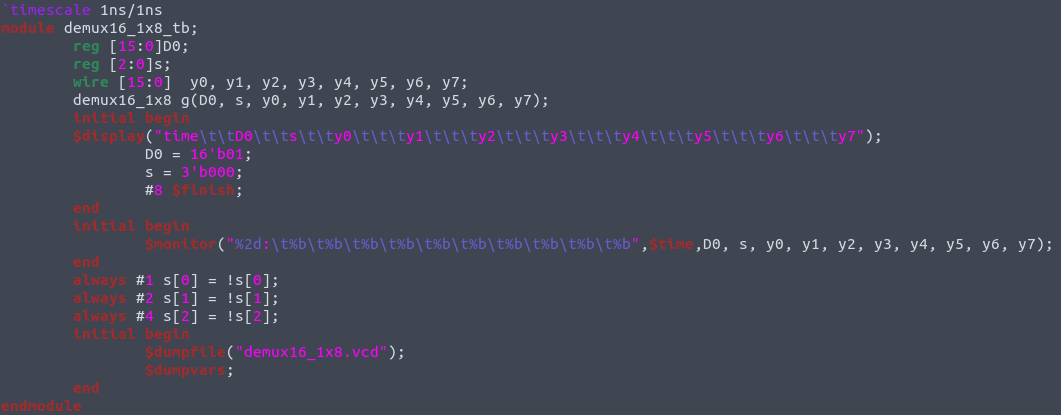
\includegraphics[scale=0.35]{16_1x8DEMUX_2.png} 
\end{figure}

La tabla de verdad corrobora lo elaborado.
\begin{figure}[h!]
\centering
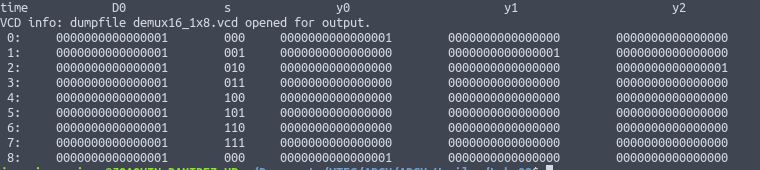
\includegraphics[scale=0.4]{16_1x8DEMUX_31.png} 
\end{figure}
\begin{figure}[h!]
\centering
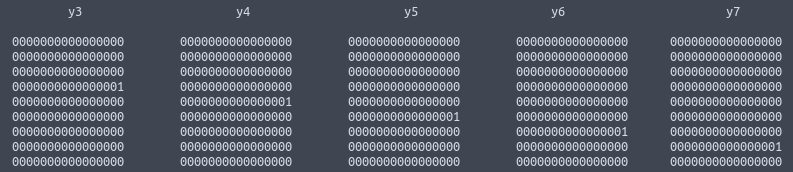
\includegraphics[scale=0.4]{16_1x8DEMUX_32.png} 
\end{figure}

\pagebreak
Con los \textit{waveforms} se puede observar que en cada tiempo solo un \textit{output} toma el valor de $D0$.
\begin{figure}[h!]
\centering
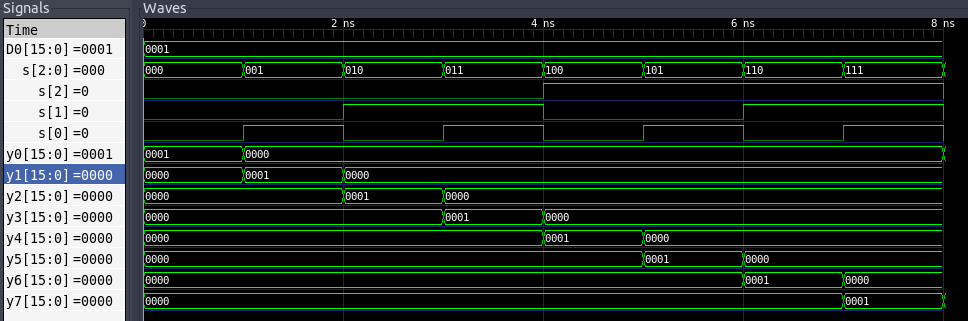
\includegraphics[scale=0.35]{16_1x8DEMUX_4.png} 
\end{figure}
\item Implementación del DEMUX 1-to-16 de 16-bits. Conforme a la misma idea de los dos ejercicios anteriores, si una determinada combinación de $selects$ se presenta para determinado output, entonces a éste se le asigna el valor de D0. De lo contrario, se le asigna un 0 de 16 bits. En este caso, el $select$ es un bus de 4 bits, con el que se pueden generar $2^4 = 16$ posibles combinaciones.
\begin{figure}[h!]
\centering
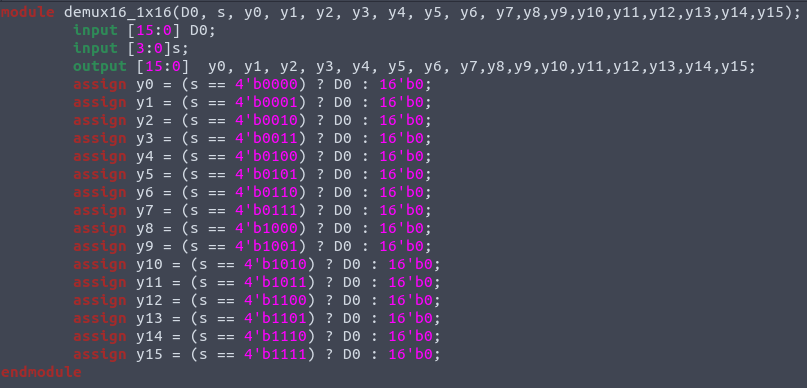
\includegraphics[scale=0.35]{16_1x16DEMUX_1.png} 
\end{figure}

En el \textit{test bench} se asignan ún valor inicial $D0 = 16'b01$. Se analizan 16 tiempos, dentro de los cuales cada se generarán todas las combinaciones de 4 bits del $select$. Esto permitirá ver que en cada tiempo, solo un output tendrá el valor de $D0$.
\begin{figure}[h!]
\centering
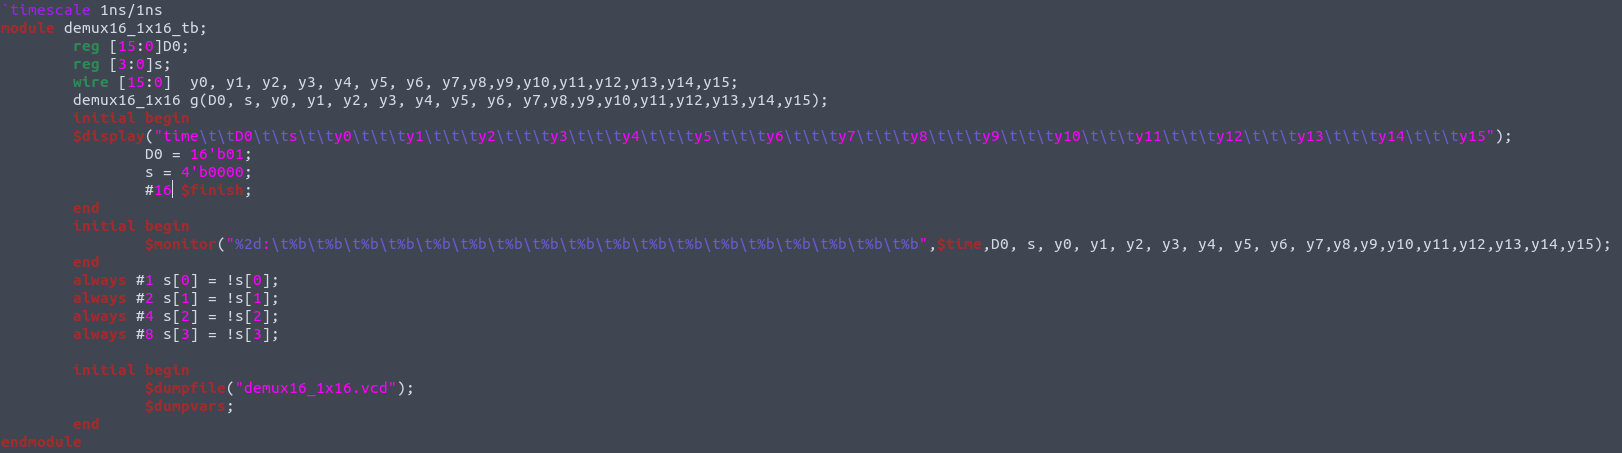
\includegraphics[scale=0.25]{16_1x16DEMUX_2.png} 
\end{figure}

La tabla de verdad confirma el planteamiento anterior.
\begin{figure}[h!]
\centering
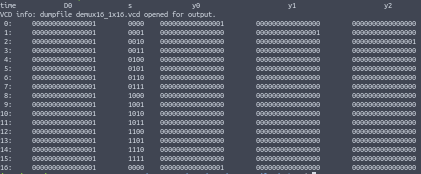
\includegraphics[scale=0.6]{16_1x16DEMUX_31.png} 
\end{figure}
\begin{figure}[h!]
\centering
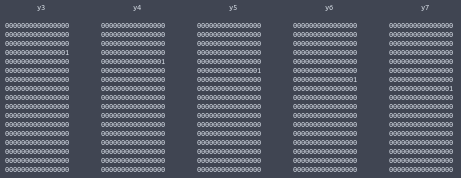
\includegraphics[scale=0.6]{16_1x16DEMUX_32.png} 
\end{figure}
\begin{figure}[h!]
\centering
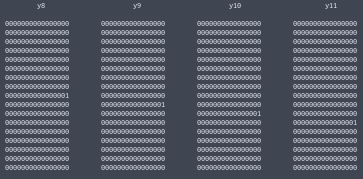
\includegraphics[scale=0.6]{16_1x16DEMUX_33.png} 
\end{figure}
\begin{figure}[h!]
\centering
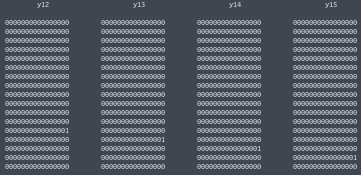
\includegraphics[scale=0.6]{16_1x16DEMUX_34.png} 
\end{figure}
\pagebreak

Los \textit{waveforms} permiten ver el cambio en determinados outputs de una manera más eficiente.
\begin{figure}[h!]
\centering
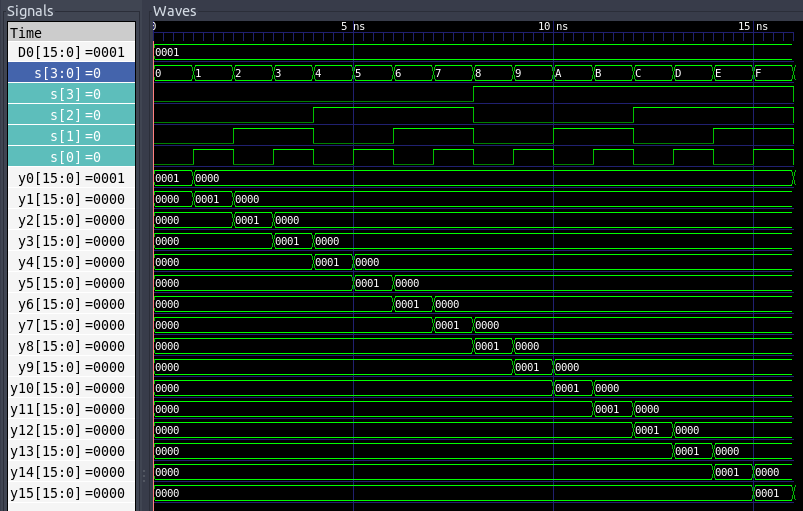
\includegraphics[scale=0.4]{16_1x16DEMUX_4.png} 
\end{figure}
\end{enumerate}
\item Implementación de un decoder 3-to-8 $(m \ - 2^m)$. Se tiene un \textit{input n} de 3 bits, cuyos 8 posibles valores indican qué posición del output de 8 bits será 1. Si se presenta una combinación de particular de $n$, entonces una posición (7:0) del output será 1, y las demás 0. Se tiene un enable que verifica antes de todo la ``autorización" del sistema. Cuando $ena =  1$, entonces proceden las validaciones de $n$. No obstante, en el caso de que $n = 0$, no es necesario ver el valor de $n$ (se toman como \textit{don't care}), pues automáticamente todas las posiciones del \textit{output} serán 0.
\begin{figure}[h!]
\centering
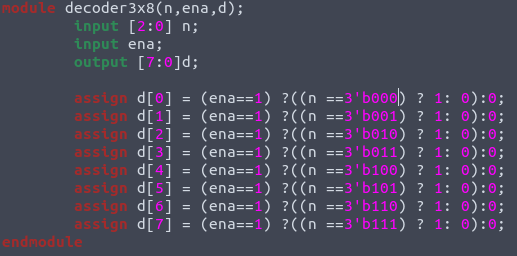
\includegraphics[scale=0.5]{decoder3x8_1.png} 
\end{figure}
\pagebreak

En el \textit{test bench}, el valor inicial de $n$ es 000. Se generarán todas las combinaciones de éste durante 8 tiempos. Esto permitirá analizar que en cada tiempo una posición diferente del \textit{output} se vuelve 1.
\begin{figure}[h!]
\centering
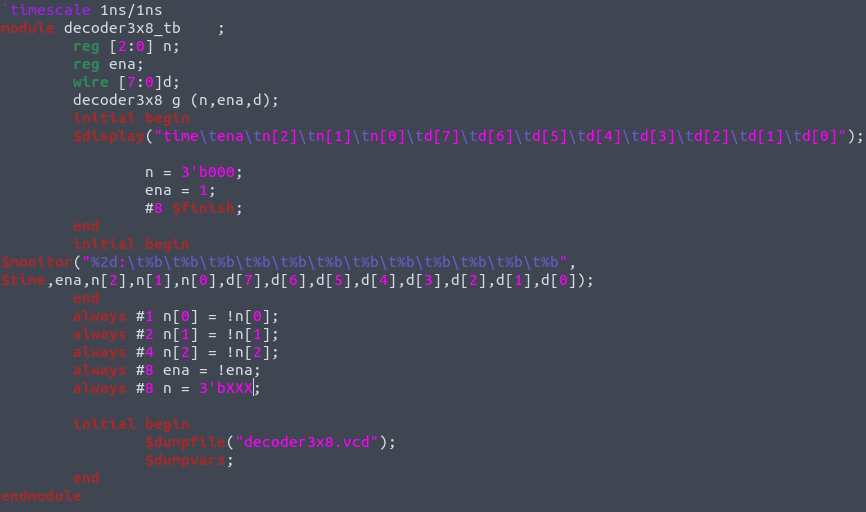
\includegraphics[scale=0.4]{decoder3x8_2.png} 
\end{figure}

En la tabla de verdad se puede ver que en cada tiempo un bit diferente de $d$ es 1, y los demás son 0. Asimismo, en el último tiempo analizado, el $enable = 0$, por lo que $n$ está lleno de \textit{don't cares}, y todos los bits de $d$ son 0.
\begin{figure}[h!]
\centering
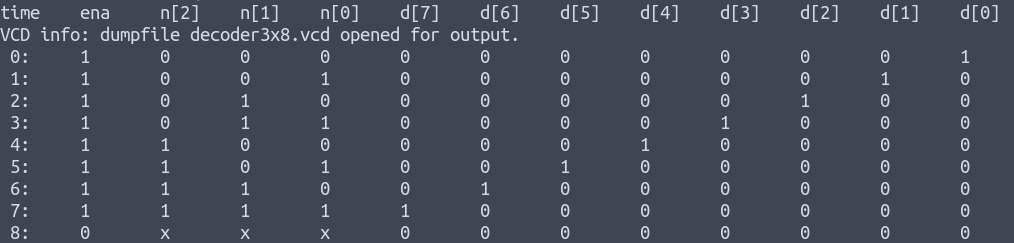
\includegraphics[scale=0.4]{decoder3x8_3.png} 
\end{figure}
\pagebreak

Los \textit{waveforms} enclarecen el cambio de 0 a 1 de un determinado bit de $d$ en cada tiempo.
\begin{figure}[h!]
\centering
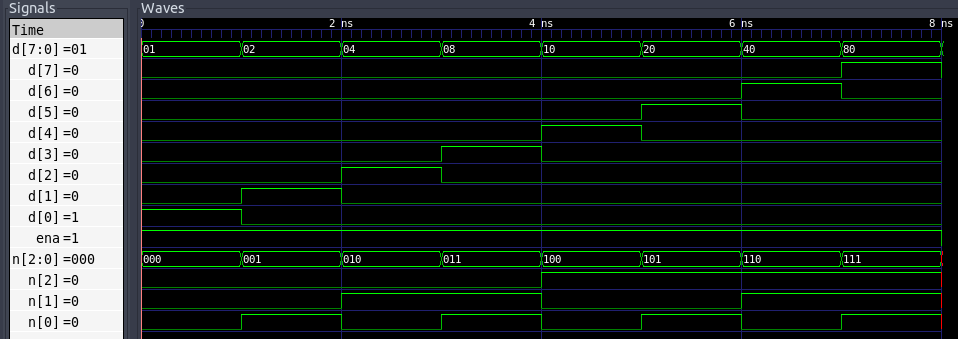
\includegraphics[scale=0.4]{decoder3x8_4.png} 
\end{figure}
\item Implementación de un\textit{priority encoder} 8-to-3. La implementación de este sistema se hizo con $casex$. Éste es un tipo particular de \textit{case statement}, que permite comparar bits ``sin importar" ciertas posiciones. En este caso, compara el input $d$ de 8 bits con 8 diferentes posibilidades, cada posición igual a 1, y las otras igual a 0. El $casex$ analiza $d$ (de izquierda a derecha) hasta encontrar un 1. El valor de los bits después del 1 no son de relevancia. Como el \textit{priority encoder} es la operación inversa del ejercicio anterior (decoder), entonces no es necesario analizar lo que viene después del 1 en $d$, pues ya se sabe que no habrá otro 1. De igual manera como antes, se asigna 000 a $n$ cuando $ena = 0$; de lo contrario, se analizan los bits.
\begin{figure}[h!]
\centering
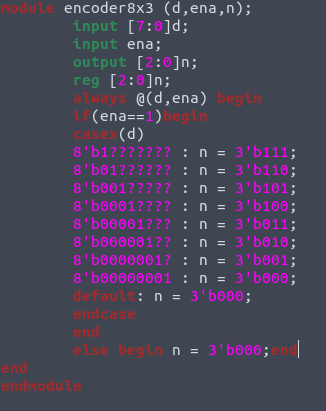
\includegraphics[scale=0.5]{encoder8x3_1.png} 
\end{figure}
\pagebreak

En el \textit{test bench} se asigna como valor inicial $d=8'b00$ y $ena=1$. Durante 8 tiempos se cambia el valor de $d$, para observar el cambio en $n$. En el noveno tiempo se asigna $ena=0$.
\begin{figure}[h!]
\centering
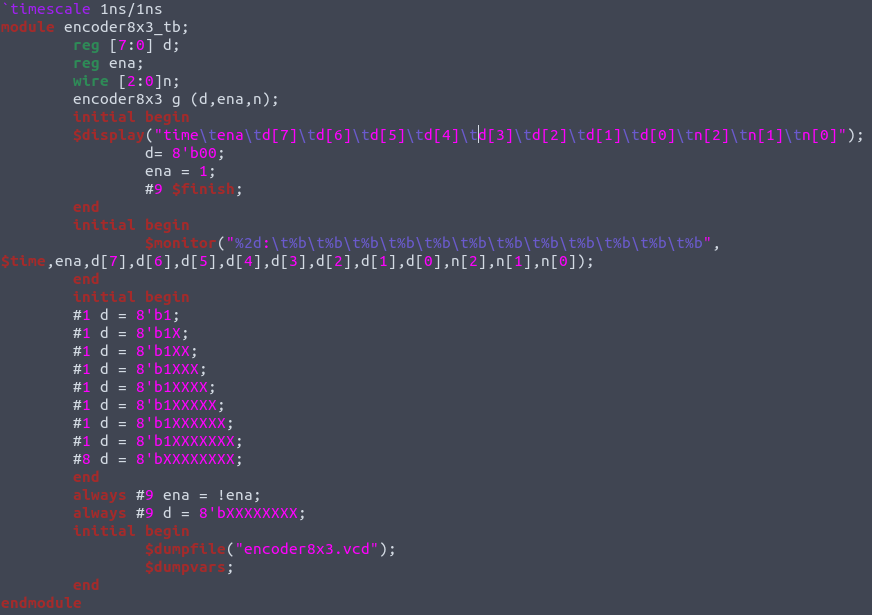
\includegraphics[scale=0.4]{encoder8x3_2.png} 
\end{figure}

La tabla de verdad verifica el comportamiento planteado del sistema.
\begin{figure}[h!]
\centering
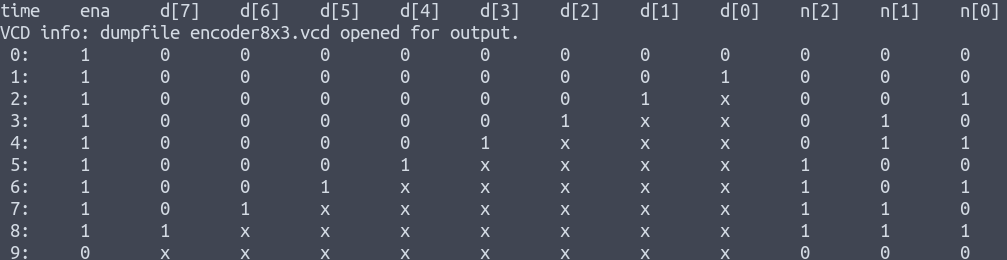
\includegraphics[scale=0.4]{encoder8x3_3.png} 
\end{figure}
\pagebreak

Los \textit{waveforms} ayudan a la visualización del cambio en los valores de cada bit de $d$, entre 0, 1 y \textit{don't care}. Para cada valor de $d$, hay un valor de $n$ diferente.
\begin{figure}[h!]
\centering
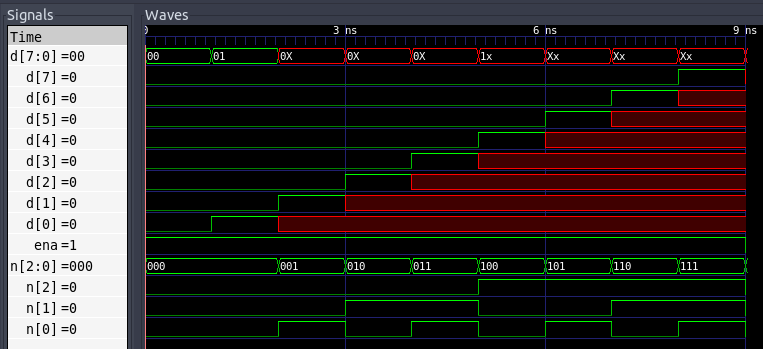
\includegraphics[scale=0.4]{encoder8x3_4.png} 
\end{figure}
\item Implementación del \textit{barrel shifter} de 32-bits. Ésta operación tiene que ser capaz de mover un \textit{input} $d$ de 32 bits hacia la derecha o izquierda, llenando los espacios vaciós con ceros o con el valor de $d[31]$. Se partió del siguiente diagrama:
\begin{figure}[h!]
\centering
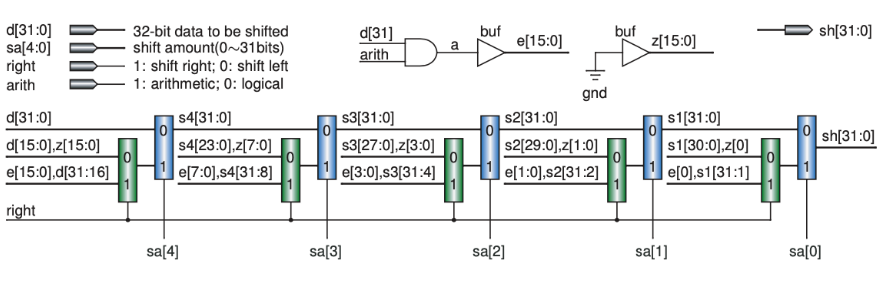
\includegraphics[scale=0.3]{barrel_diagram.png} 
\end{figure}

Primero se construye un \textit{wire} $e$, a través del módulo ANDE. Cuando $arith = 1$, entonces $e$ toma el valor de $d[31]$, concatenado 16 veces. En el caso contrario, $e = 16'b00$. 
\begin{figure}[h!]
\centering
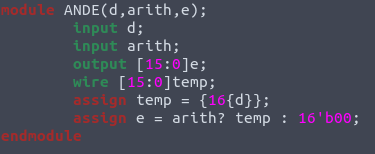
\includegraphics[scale=0.4]{barrelshifter_11.png} 
\end{figure}
\pagebreak

Después se genera el módulo mux32 2x1, que se utilizará 10 veces a lo largo del \textit{shifter}. Si el \textit{select s} es 0, entonces el \textit{wire y} tomará el valor de $a$. De lo contrario, tomará el valor de $b$.
\begin{figure}[h!]
\centering
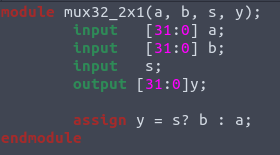
\includegraphics[scale=0.5]{barrelshifter_12.png} 
\end{figure}

En el \textit{.v} se ``llaman" a los módulos previamente indicados siguiendo el ``camino" del diagrama anterior. El \textit{input sa} de 5 bits contiene los \textit{selects} que se usarán a lo largo del \textit{shifter}. Después de que los 10 MUX se ``ejecuten", el valor final de la operación es asignado a $sh$.
\begin{figure}[h!]
\centering
\includegraphics[scale=0.4]{barrelshifter_1.png} 
\end{figure}
\pagebreak

En el \textit{test bench} se asigna el valor inicial $d =$ 11111111000000000 000000011111111. Se desea que se ``muevan" los bits en bloques de 8, entonces $sa = 5'b100$. Para poder ver todas las posibilidades de \textit{shifts}, se inicia con $right = 0$ y $arith = 0$, y durante 3 tiempos se realizan todas las combinaciones indicadas en la tarea, para poder ver como cambia $sh$.
\begin{figure}[h!]
\centering
\includegraphics[scale=0.4]{barrelshifter_2.png} 
\end{figure}

A través de la tabla de verdad se pueden observar cómo se dan los movimientos. En el tiempo 1, hay un \textit{right logicalic shift}, porque se mueve a la derecha y se rellenan los espacios vacíos con ceros. En el tiempo 2, hay un \textit{right arithmetic shift}, ya que se mueve a la derecha y se replica $d[31]$ en las posiciones vacías. Finalmente, en el tiempo 3 hay un \textit{left logical shift}, pues se mueve a la izquierda y se llenan los espacios vacíos con ceros.
\begin{figure}[h!]
\centering
\includegraphics[scale=0.4]{barrelshifter_3.png} 
\end{figure}
\pagebreak

A través de los \textit{waveforms} se puede apreciar cómo cambian de valor ciertos bits de $sh$. Se ven con claridad los \textit{shifts}. 
\begin{figure}[h!]
\centering
\includegraphics[scale=0.4]{barrelshifter_4.png} 
\end{figure}
\end{enumerate}
\end{document}